% !TEX root = ../main.tex

\begin{frame}{Telephone}
	\begin{columns}[T,onlytextwidth]
		\column{0.5\textwidth}
		\begin{figure}
			\centering
			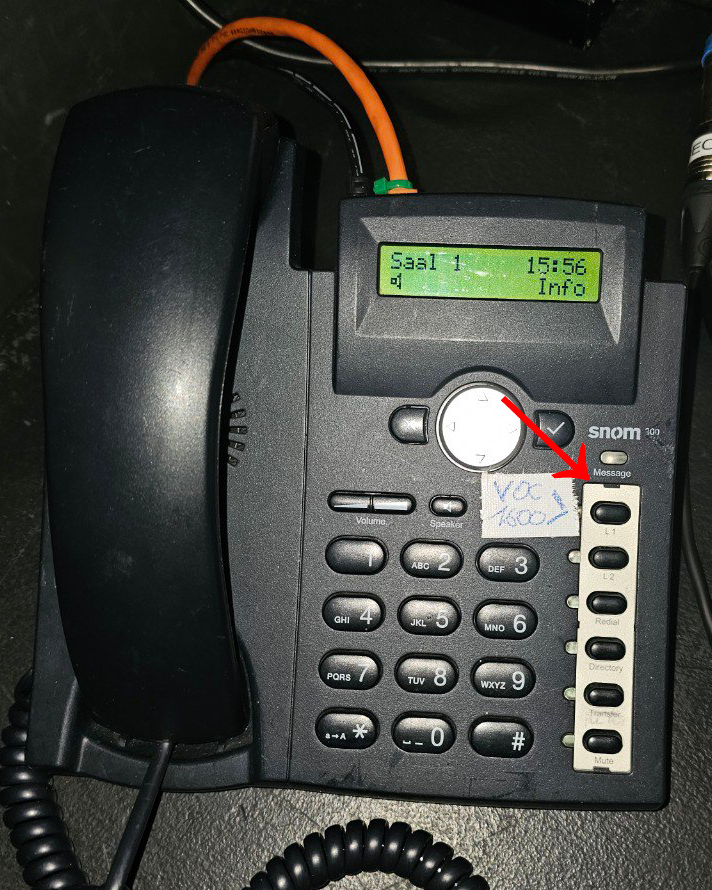
\includegraphics[width=0.5\textwidth]{images/telephone.png}
			\caption{Telephone on Mixer Desk}
		\end{figure}
		\column{0.5\textwidth}
		\begin{itemize}
		\item If there are any issues, contact us via Telephone. Just press the VOC Button (red arrow)
		\item Call us via DECT 1601 and state the lecture hall you are in.
		\end{itemize}

	\end{columns}
\end{frame}

\begin{frame}{Intercom: Mixer}
	\begin{columns}[T,onlytextwidth]
		\column{0.5\textwidth}
		\begin{figure}
			\centering
			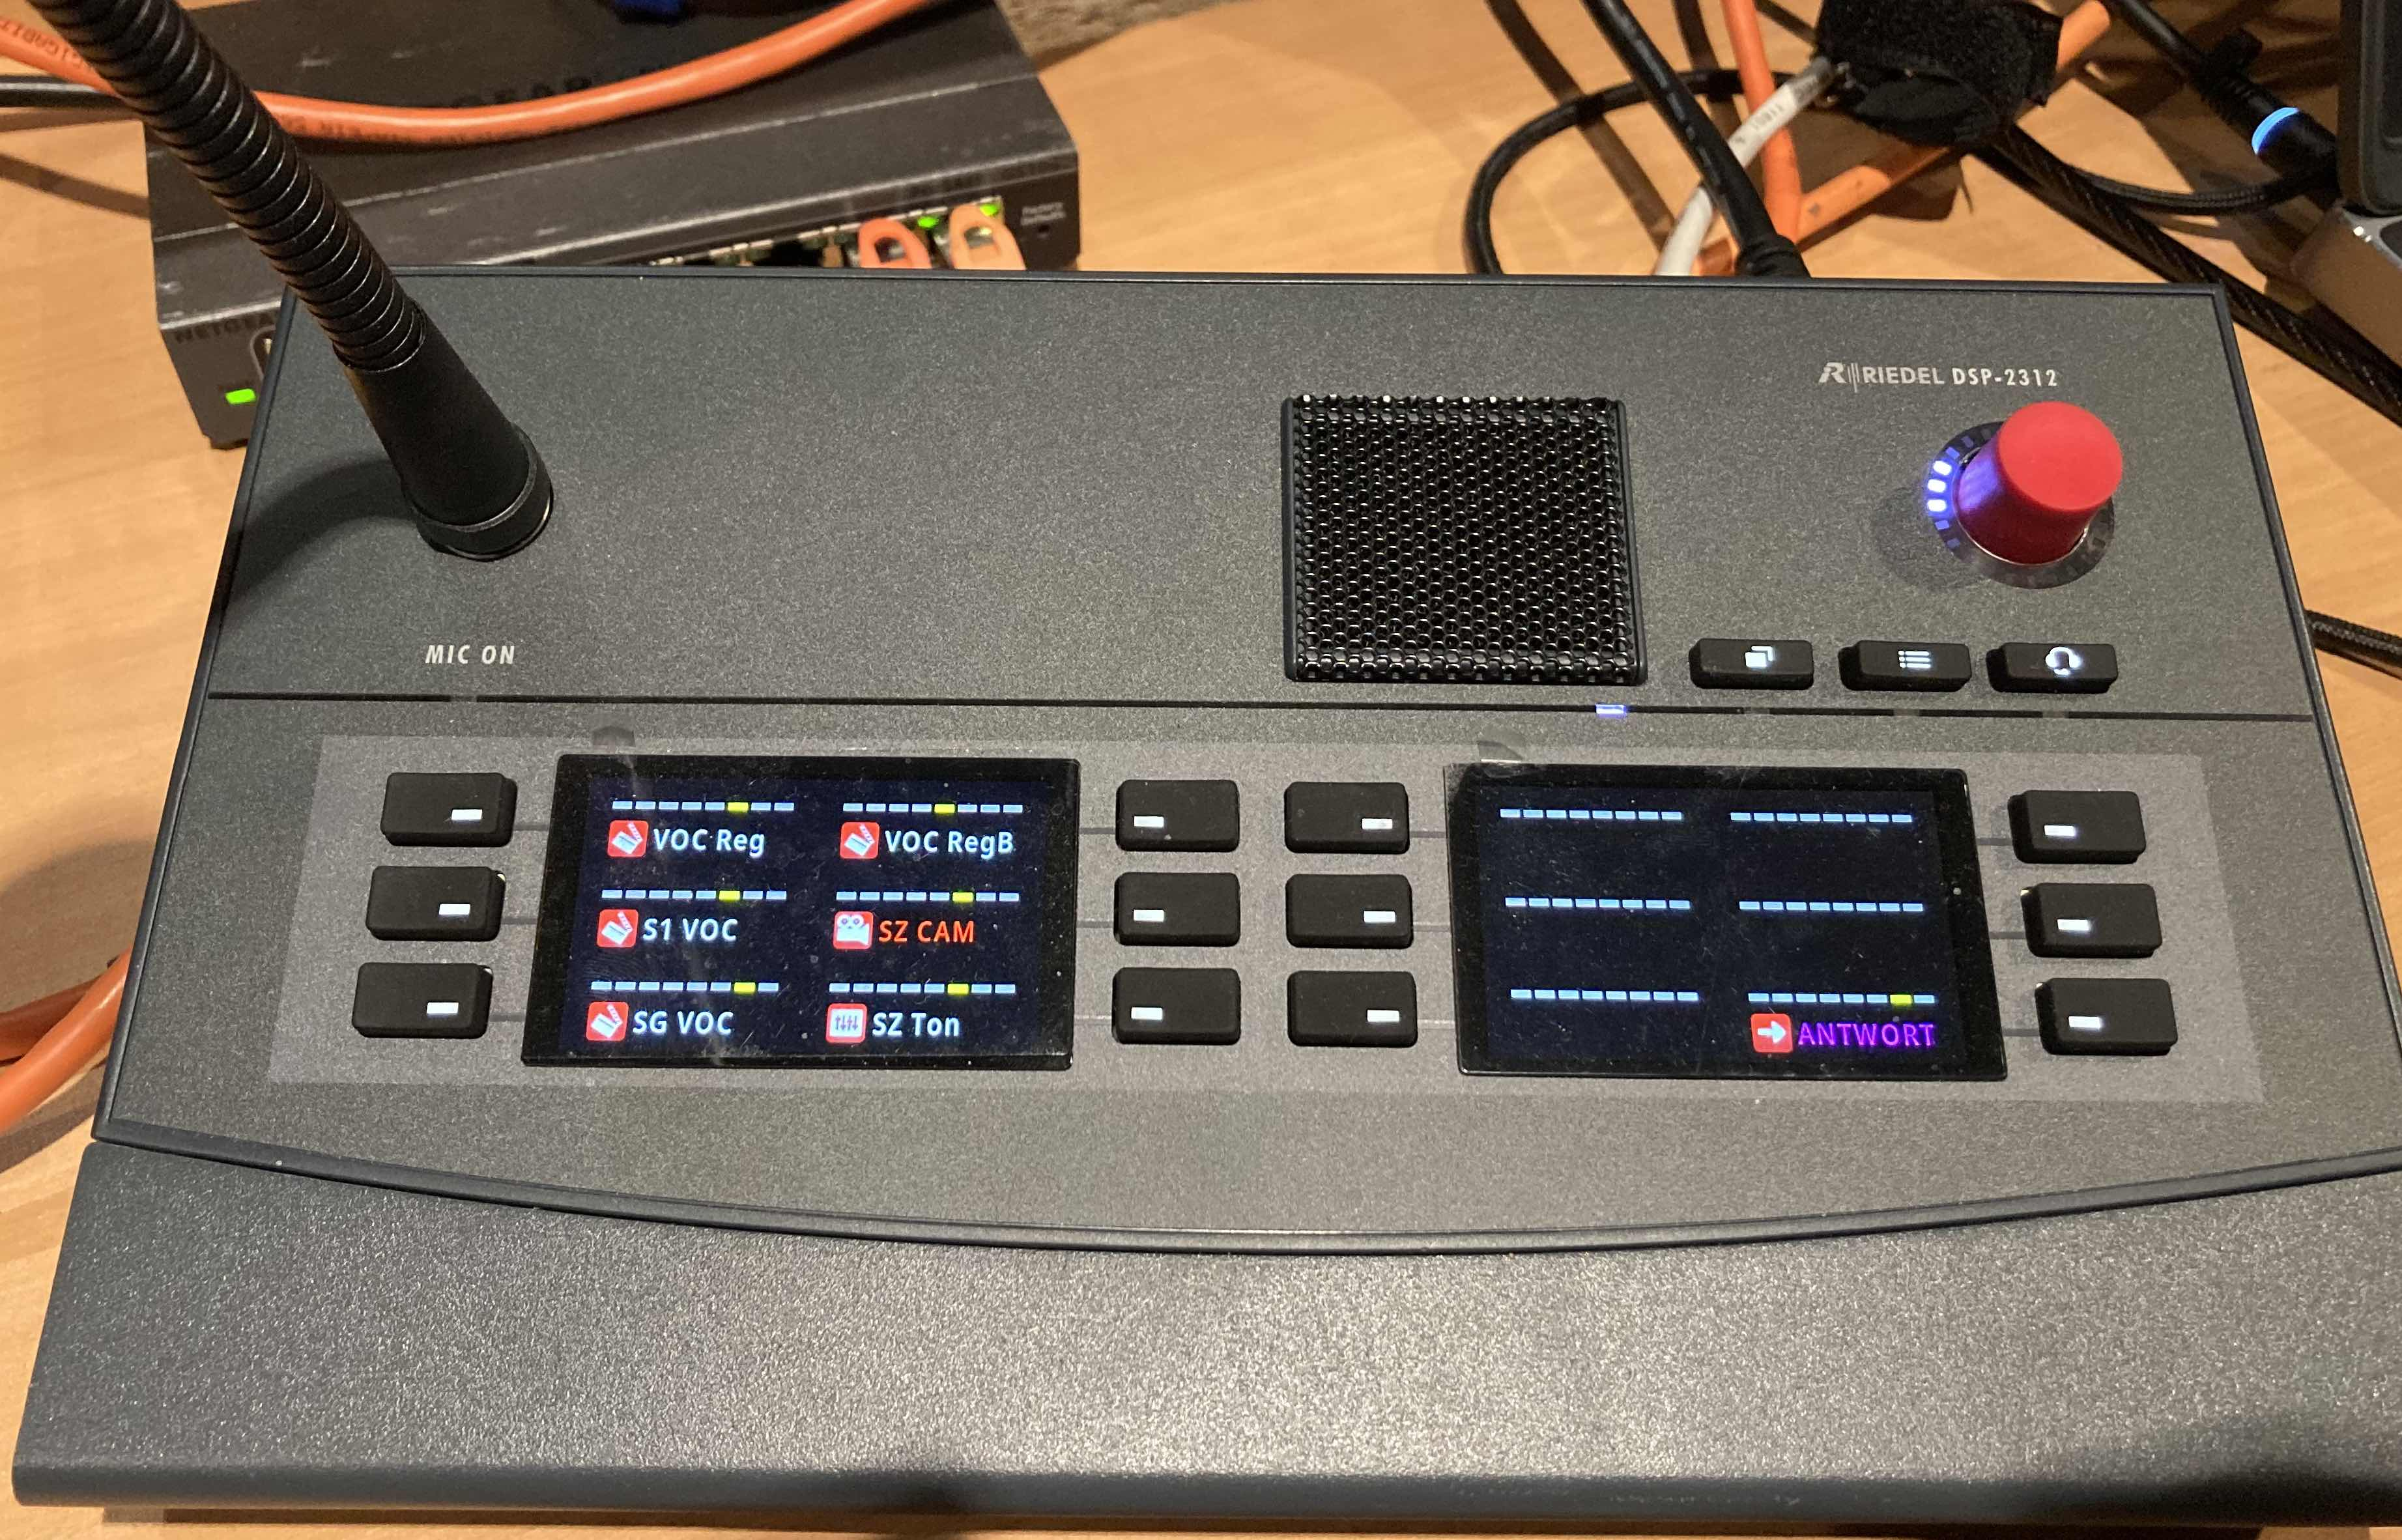
\includegraphics[width=0.9\textwidth]{images/intercom-riedel-panel.jpg}
			\caption{Intercom Device: Main Station}
		\end{figure}
		\column{0.5\textwidth}
			We use a party-line style intercom for communication between mixer and camera
		\begin{itemize}
			\item Press the button next to "CAM" to talk to cameras
			\item Touch channel and turn red knob to adjust volume
		\end{itemize}
	\end{columns}
\end{frame}

\begin{frame}{Intercom: Camera}
	\begin{columns}[T,onlytextwidth]
		\column{0.5\textwidth}
		\begin{figure}
			\centering
			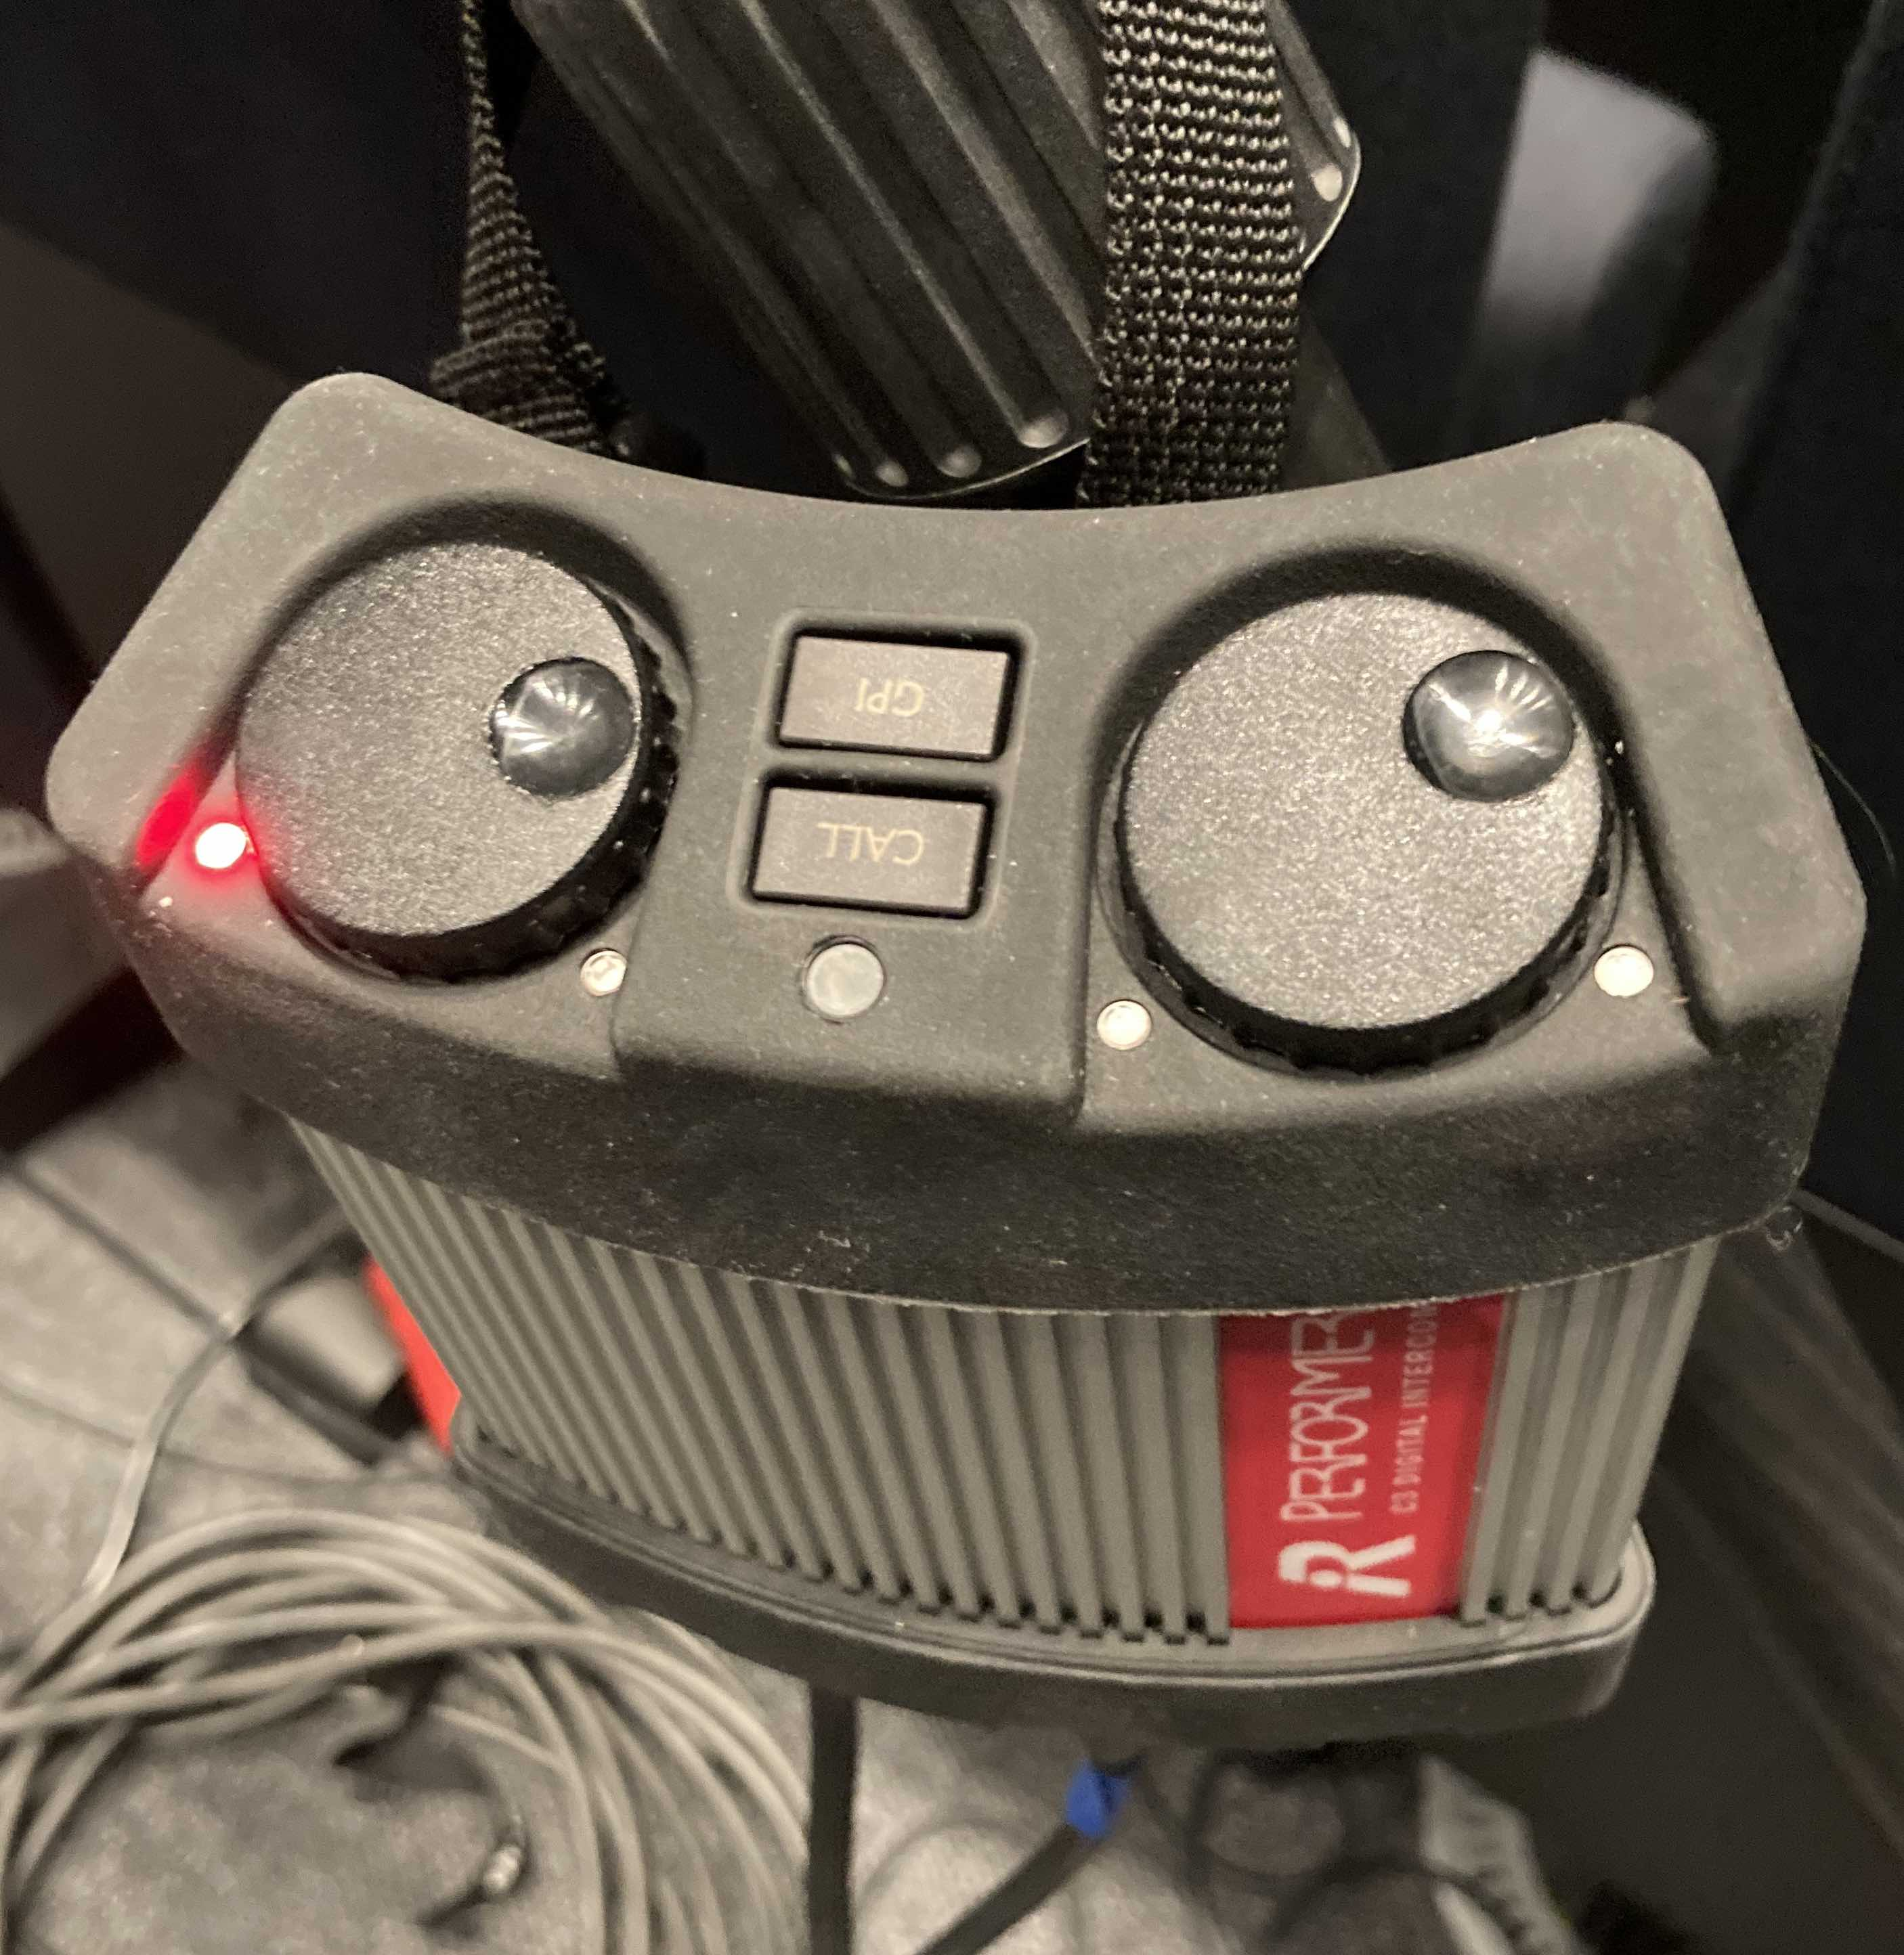
\includegraphics[width=0.75\textwidth]{images/intercom-riedel-beltpack.jpg}
			\caption{Intercom Device: Camera Station}
		\end{figure}
		\column{0.5\textwidth}

		\begin{itemize}
			\item Press right button to talk
			\item Turn knob to adjust headphone volume
			\item Red light is an inactive channel!
		\end{itemize}
	\end{columns}
\end{frame}
